In this section, we demonstrate the performance and capability of Bempp-Exafmm via electrostatic simulations, including computing the solvation energy of Zika virus.
We ran all experiments on a single CPU node of Pegasus, equipped with two 20-core Intel Xeon Gold 6148 CPUs running at 3.7 GHz and 192GB RAM.
All runs are based on Bempp-cl version 0.2.2.
We compiled Exafmm with Intel compiler (version 19.0.5.281) and enabled \texttt{-xHost} option for vectorization.

\subsection{Mesh refinement study using a spherical molecule}

To verify our \bem-\fmm integration, we first performed a mesh refinement study for a spherical molecule with an off-center charge.
Figure \ref{fig:sketch_sphere_convergence} depicts the problem setup.
The molecule has a radius of 4 Angstrom and a relative permittivity of $\epsilon_1 = 4$; the unit charge is located at $(1,1,1)$.
The solvent region has a relative permittivity of water ($\epsilon_2 = 80$); and the salt concentration is set to $150mM$ $(\kappa = 1/8 {\si{\angstrom}}^{-1})$.
Other simulation parameters are listed in Table \ref{tab:sim_params_convergence}.
We compute the solvation energy of this molecule using $5$ meshes with a constant refinement factor of 4.

\begin{figure}[htbp]
    \centering
    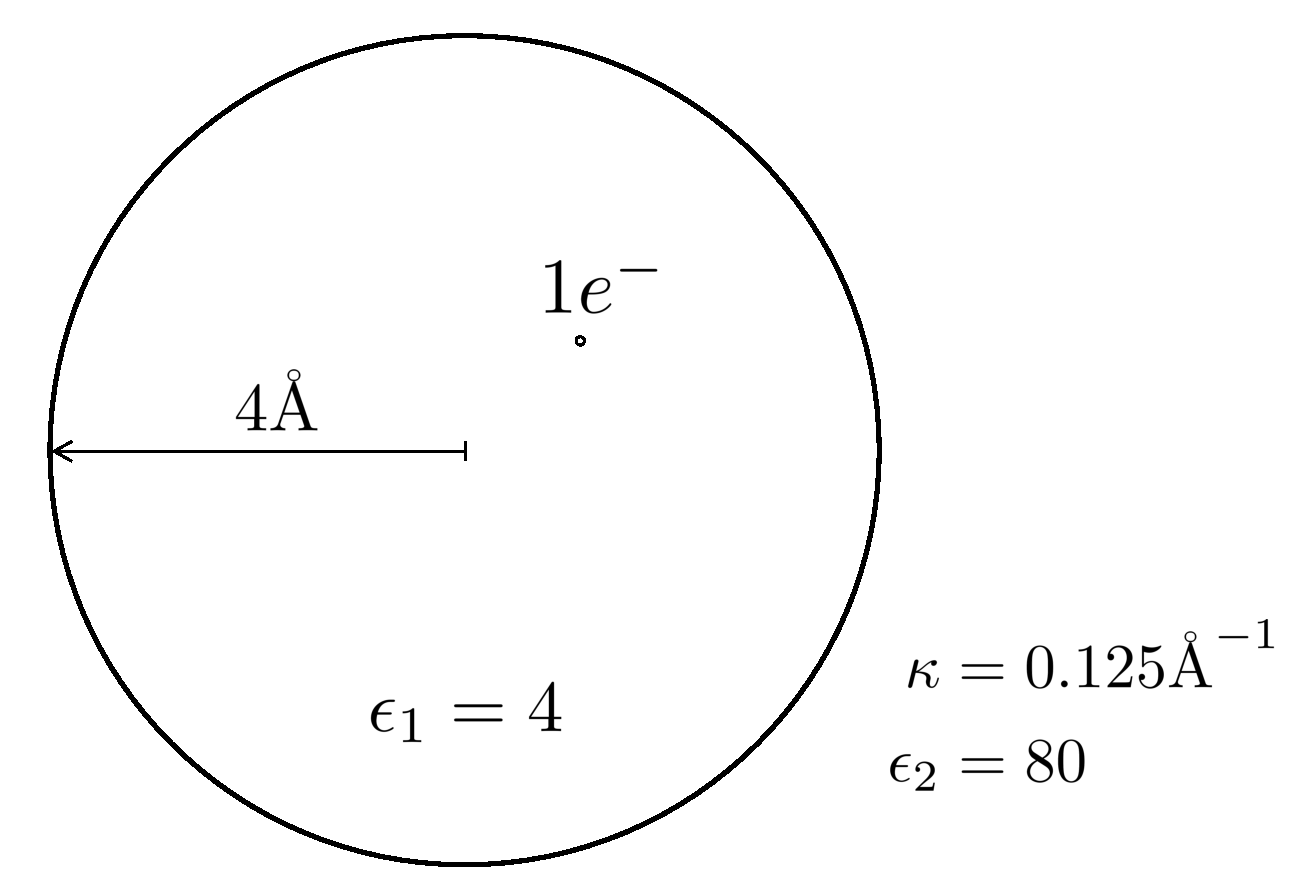
\includegraphics[width=0.8\linewidth]{sketch_sphere_convergence.pdf}
    \caption{Sketch of a spherical molecule with an off-center unit charge at $(1,1,1)$.}
    \label{fig:sketch_sphere_convergence}
\end{figure}

\begin{table}[]
    \centering
    \begin{tabular}{lc}
    \hline
    \gmres tolerance          & $10^{-7}$ \\
    regular quadrature order  & 4    \\
    \fmm expansion order      & 10   \\
    \fmm $\ncrit$             & 500  \\
    \hline
    \end{tabular}
    \caption{Simulation parameters used in the mesh refinement study for a spherical molecule.}
    \label{tab:sim_params_convergence}
\end{table}

Kirkwood's derivation allows us to compute the analytical solution of the solvation energy for this spherical molecule: $-12.258363$ [kcal/mol],
with which we can compare our results. Figure \ref{fig:sphere_convergence} shows the error of the solvation energy converges at the expected rate of $1/N$ for both formulations.

\begin{figure}[htbp]
    \centering
    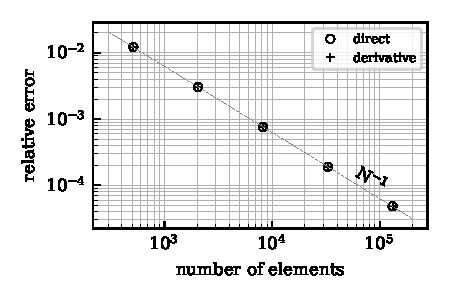
\includegraphics[width=\linewidth]{sphere_convergence.pdf} 
    \caption{Mesh convergence study of the solvation energy of a spherical molecule with an off-center charge, using both direct formulation and Juffer's formulation. The error is with respect to the analytical solution. 
    The sphere is discretized with 512, 2048, 8192, 32768 and 131072 boundary elements.}
    \label{fig:sphere_convergence}
\end{figure}

\subsection{Mesh refinement study using 5PTI}

Next, we tested our code on a realistic structure - bovine pancreatic trypsin inhibitor (PDB code 5PTI), whose structure is shown in Figure \ref{fig:5PTI_structure}.
Similarly, we compute its solvation energy using 5 meshes with the element density ranging from 1 to 16 (Table \ref{tab:5PTI_mesh}).
Same fine parameters in Table \ref{tab:sim_params_convergence}, were used as the previous test, to reveal the discretization error.
Since an analytical solution is not available for this geometry, the reference values for error estimation come from Richardson extrapolation.

\begin{figure}[htbp]
    \centering
    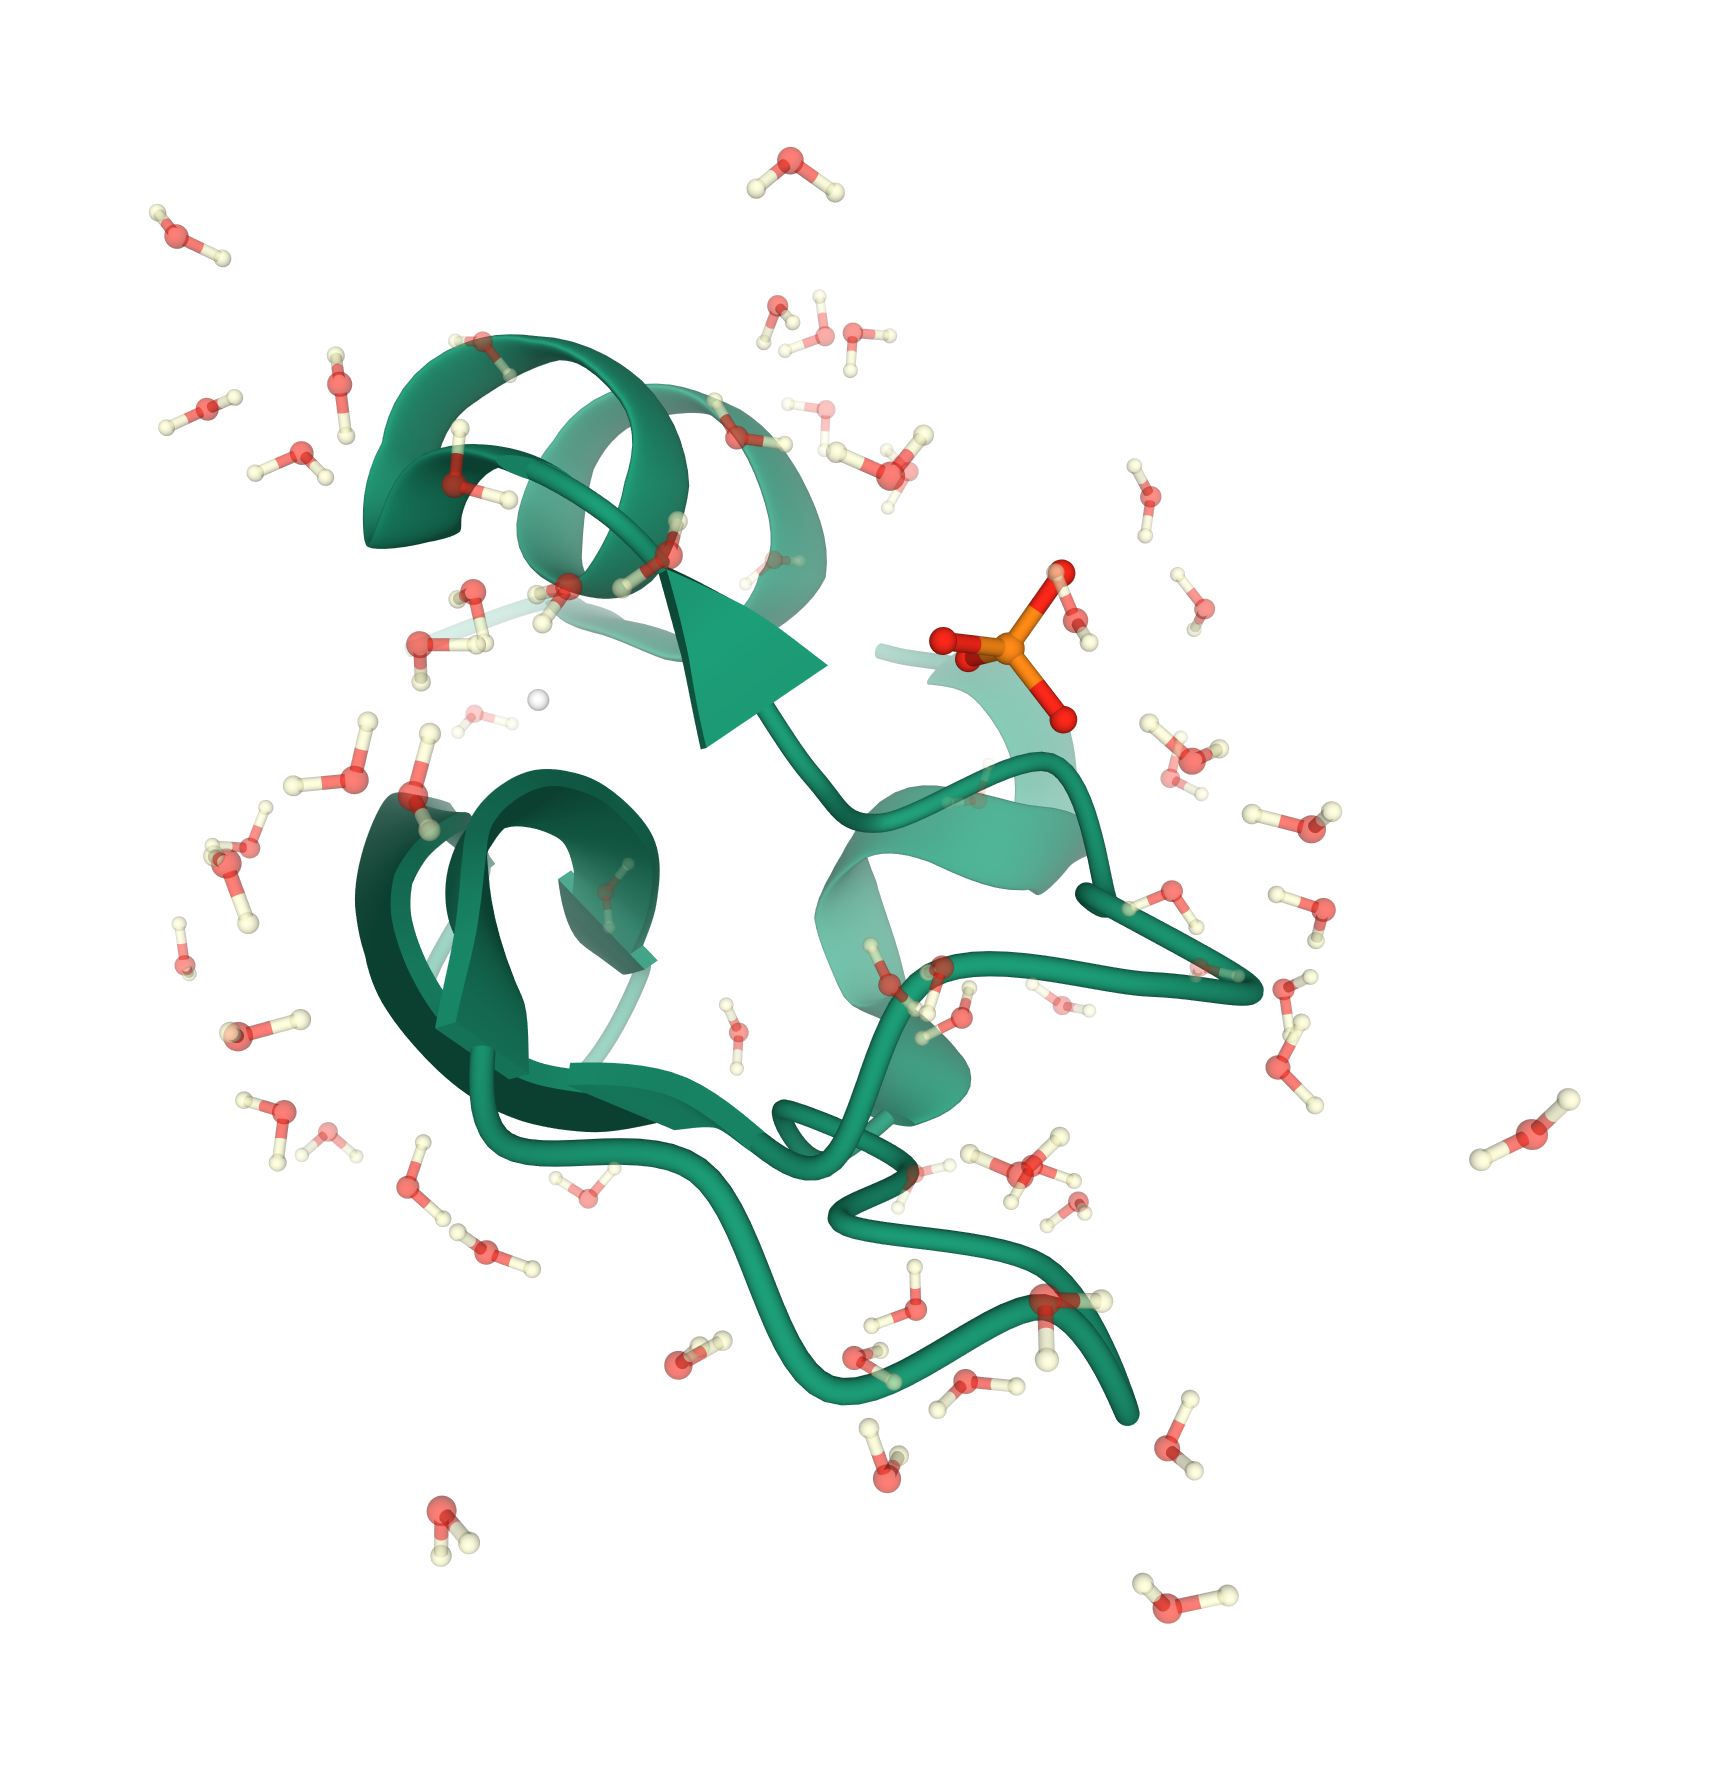
\includegraphics[width=\linewidth]{5PTI.png}
    \caption{Structure of bovine pancreatic trypsin inhibitor (PDB code 5PTI).}
    \label{fig:5PTI_structure}
\end{figure}

\begin{table}[]
    \centering
    \begin{tabular}{cc}
    number of elements & mesh density ($\#/{\si{\angstrom}}^2$) \\
    \hline
    3032               & 1                                       \\
    6196               & 2                                       \\
    12512              & 4                                       \\
    25204              & 8                                       \\
    50596              & 16                                     
    \end{tabular}
    \caption{Mesh sizes and mesh densities of 5 meshes used in the grid refinement study on 5PTI. Mesh densities are measured by the number of elements per square Angstrom.}
    \label{tab:5PTI_mesh}
\end{table}

Figure \ref{fig:5PTI_convergence} shows that the error of computing solvation energy of 5PTI converges linearly with respect to $N$, for both direct and Juffer's formulation.
Both convergence results confirm that our software solves the mathematical model correctly.

\begin{figure}[htbp]
    \centering
    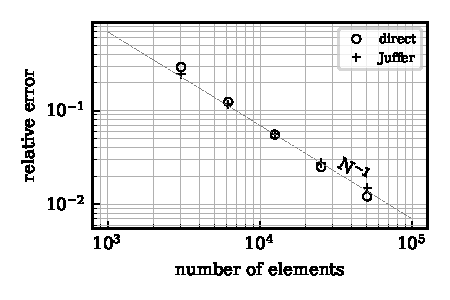
\includegraphics[width=\linewidth]{5PTI_convergence.pdf} 
    \caption{Mesh convergence study of the solvation energy of bovine pancreatic trypsin inhibitor (PDB code 5PTI), using both direct formulation and Juffer's formulation.
    The error is with respect to the extrapolated solution using Richardson extrapolation.}
    \label{fig:5PTI_convergence}
\end{figure}

\subsection{Performance study using a spherical molecule}

In this section, we investigate the performance of Bempp-Exafmm using a spherical molecule.
The sphere has a radius of 1; 100 charges are placed randomly inside, representing the atoms in the solute.
We used the same dielectric constants and salt concentration as in previous the grid-convergence study.
Other simulation parameters are reported in Table \ref{tab:sim_params_performance}.

\begin{table}[]
    \centering
    \begin{tabular}{lc}
    \hline
    \gmres tolerance          & $10^{-4}$ \\
    regular quadrature order  & 4    \\
    \fmm expansion order      & 5   \\
    \fmm $\ncrit$             & 500  \\
    \hline
    \end{tabular}
    \caption{Simulation parameters used in the performance study for a spherical molecule.}
    \label{tab:sim_params_performance}
\end{table}

To imitate a wide range of problem sizes, we used five surface discretizations, with the number of elements ranging from 8 thousand to 2 million.
Table \ref{tab:sphere_time} presents the assembly time, the solution time and the number of iterations to converge in each case for both direct and Juffer's formulation.
The convergence results show that the condition number grows as the problem size increases in direct formulation; while it remains at the same level in Juffer's formulation.

\begin{table*}[]
    \centering
    \begin{tabular}{c|cccc|cccc}
                                                                 & \multicolumn{4}{c|}{direct}                                                                                                                                                                       & \multicolumn{4}{c}{Juffer}                                                                                                                                                                        \\ \hline
    \begin{tabular}[c]{@{}c@{}}number of\\ elements\end{tabular} & \begin{tabular}[c]{@{}c@{}}total\\ time (s)\end{tabular} & \begin{tabular}[c]{@{}c@{}}assembly\\ time (s)\end{tabular} & \begin{tabular}[c]{@{}c@{}}GMRES\\ time (s)\end{tabular} & \# iterations & \begin{tabular}[c]{@{}c@{}}total\\ time (s)\end{tabular} & \begin{tabular}[c]{@{}c@{}}assembly\\ time (s)\end{tabular} & \begin{tabular}[c]{@{}c@{}}GMRES\\ time (s)\end{tabular} & \# iterations \\ \hline
    8192                                                         & 14.0                                                     & 5.4                                                         & 8.6                                                      & 20            & 15.2                                                     & 9.4                                                         & 5.8                                                      & 4            \\
    32768                                                        & 35.1                                                     & 11.7                                                        & 23.4                                                     & 24            & 36.8                                                     & 22.5                                                        & 14.3                                                     & 4            \\
    131072                                                       & 144.2                                                    & 32.8                                                        & 111.4                                                    & 34            & 116.9                                                    & 68.6                                                        & 48.3                                                     & 4            \\
    524288                                                       & 675.8                                                    & 121.6                                                       & 554.2                                                    & 51            & 437.9                                                    & 276.0                                                       & 161.9                                                    & 4            \\
    2097152                                                      & 3159.8                                                   & 483.3                                                       & 2676.5                                                   & 70            & 1809.8                                                   & 1237.0                                                      & 572.8                                                    & 4           
    \end{tabular}
    \caption{Assembly and solution times of calculating the solvation energy of a spherical molecule with 100 random charges inside.
    Assembly time include time spent on preparing preconditioners.}
    \label{tab:sphere_time}
\end{table*}

In our implementation, each iteration in direct formulation requires $8$ \fmm evaluations, whereas each iteration in Juffer's formulation requires 19, making it more than twice as expensive.
That explains why the direct formulation leads to a shorter solution time (\gmres time), despite a slower convergence, in the two smaller cases.
For larger problem sizes, faster convergence in Juffer's formulation offsets the larger cost per iteration.

Juffer's formulation always takes more time in matrix assembly.
With $2,097,152$ panels, it is $2.5$x slower than using direct formulation.
There are two reasons.
On one hand, the system matrix in Juffer's formulation requires two hypersingular operators, thus is more involved.
On the other hand, the assembly time also includes the time spent on preparing preconditioners.
Calculating the mass-matrix preconditioner used in Juffer's formulation is much more cumbersome than the block-diagonal preconditioner used in direct formulation.

Figure \ref{fig:sphere_assembly_time} shows the linear scaling of the assembly time with respect to $N$.
In fact, all the steps in matrix assembly scale linearly except for the sparse LU-decomposition required in computing the mass-matrix preconditioner for Juffer's formulation.
It explains why the slope between the last two triangles is slightly steeper than $\mathcal{O}(N)$.

\begin{figure}[htbp]
    \centering
    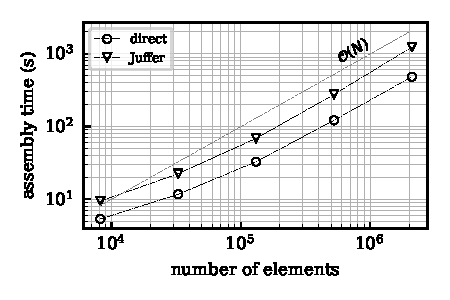
\includegraphics[width=\linewidth]{sphere_assembly_time.pdf} 
    \caption{Assembly time with respect to problem size $N$ for a spherical molecule with 100 random charges inside.}
    \label{fig:sphere_assembly_time}
\end{figure}

Next, we want to confirm that the time complexity of mat-vecs in \gmres is also $\mathcal{O}(N)$.
As we mentioned before, each iteration involves multiple \fmm evaluations: 4 Laplace {\fmm}s and 4 modified Helmholtz {\fmm}s for direct formulation, 8 and 11 for Juffer's formulation.
We averaged the time spent on 1 Laplace \fmm and 1 modified Helmholtz \fmm respectively using direct formulation, and plot them with respect to $N$ in Figure \ref{fig:sphere_fmm}.
The linear scaling substantiates the efficiency of our \fmm implementation.

\begin{figure}[htbp]
    \centering
    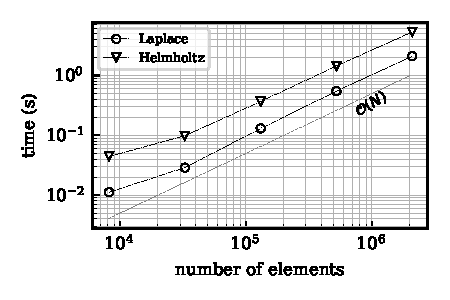
\includegraphics[width=\linewidth]{sphere_fmm.pdf} 
    \caption{The average time of 1 Laplace FMM evaluation and 1 modified Helmholtz evaluation in GMRES with respect to problem size N using direct formulation.}
    \label{fig:sphere_fmm}
\end{figure}

In Bempp, pre-computing of the invariant matrices in \fmm, initializing singular assemblers and many other computations are triggered by calling the iterative solver.
In addition, each \fmm evaluation in \gmres is followed by a singular correction which compensates the singular integrals that are not ignored by \fmm.
Therefore, the \gmres time reported here also reflects these contributions.
Figure \ref{fig:sphere_gmres} demonstrates the time breakdown of \gmres in percentage.
As problem size increases, \fmm evaluations dominate solution time.

\begin{figure}[htbp]
    \begin{subfigure}{\columnwidth}
        \centering
        \makebox[\textwidth][c]{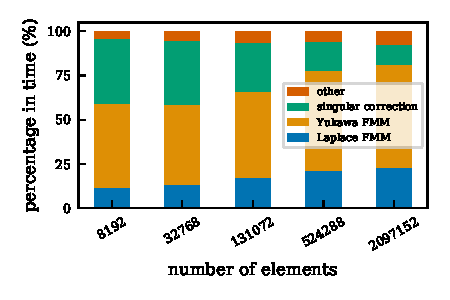
\includegraphics[width=\linewidth]{sphere_gmres_direct.pdf}}
    \end{subfigure}

    \begin{subfigure}{\columnwidth}
        \centering
        \makebox[\textwidth][c]{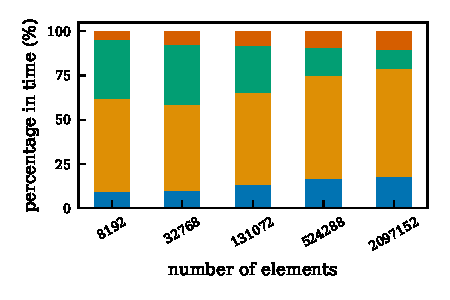
\includegraphics[width=\linewidth]{sphere_gmres_juffer.pdf}}
    \end{subfigure}

    \caption{Time breakdown of \gmres in percentage using direct formulation (top) and Juffer's formulation (bottom).}
    \label{fig:sphere_gmres}
\end{figure}

We also measured the amount of memory taken by the simulations, using the Linux command \texttt{/usr/bin/time -v}.
We observed a linear space complexity as shown in Figure \ref{fig:sphere_memory}.
The largest case, with more than $2$ million elements, requires $36$GB for direct formulation and $46$GB for Juffer's formulation.

\begin{figure}[htbp]
    \centering
    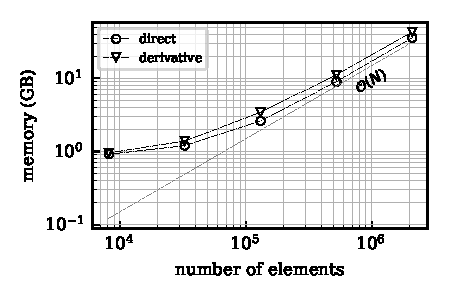
\includegraphics[width=\linewidth]{sphere_memory.pdf} 
    \caption{Overall memory consumption in GB for both direct and Juffer's formulation.}
    \label{fig:sphere_memory}
\end{figure}

\subsection{Free energy of Zika virus}

Finally, we present a more challenging problem that studies the free energy of the Zika virus (PDB code 6CO8), whose structure is shown in Figure \ref{fig:6CO8_assembly}.
We acquired the molecular structure from Protein Data Bank (PDB), parameterized it with \texttt{pdb2pqr} and generated mesh on the solvent-excluded surface using \texttt{Nanoshaper}.
The prepared structure contains about 1.6 million atoms and our mesh has around 10 million boundary elements.
In this experiment, 3 quadrature points were used for regular Galerkin integrals over disjoint elements.
The \fmm expansion order was 4 and the tolerance of \gmres was $10^{-4}$.

\begin{figure}[htbp]
    \centering
    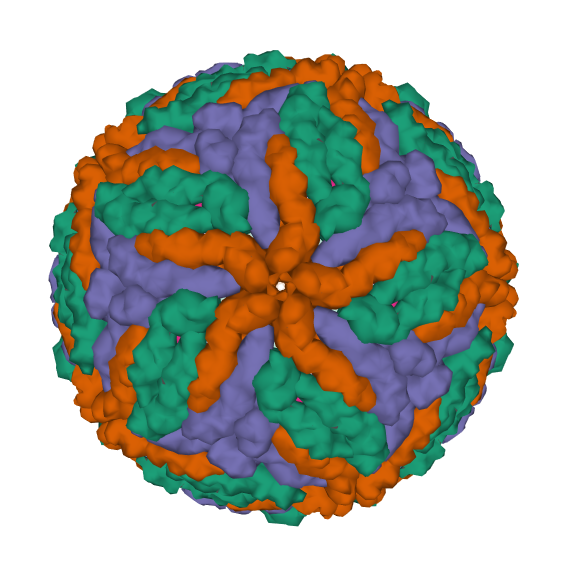
\includegraphics[width=0.8\linewidth]{6CO8_assembly.png} 
    \caption{Structure of Zika virus (PDB code 6CO8) in assembly view. Each color indicates a polymer chain.}
    \label{fig:6CO8_assembly}
\end{figure}

\begin{table*}[]
    \centering
    \begin{tabular}{c|c|ccccc}
                 & \begin{tabular}[c]{@{}c@{}}$\Delta G_{\mathrm{solv}}$\\ (kcal/mol)\end{tabular} & \begin{tabular}[c]{@{}c@{}}total \\ time (s)\end{tabular} & \begin{tabular}[c]{@{}c@{}}assembly \\ time (s)\end{tabular} & \begin{tabular}[c]{@{}c@{}}GMRES \\ time (s)\end{tabular} & \begin{tabular}[c]{@{}l@{}}memory\\ (GB)\end{tabular} & \# iterations \\ \hline
    Bempp direct & -116587.5                                                   & 11005.4                                                   & 1534.5                                                       & 9470.9                                                    & 111.8                                                 & 105           \\
    Bempp Juffer & -116255.4                                                   & 12776.2                                                   & 7766.8                                                       & 5009.4                                                    & 172.8                                                 & 17            \\
    \pygbe       & -117261.1                                                   & -                                                         & -                                                            & -                                                         & -                                                     & -            
    \end{tabular}
    \caption{Bempp and \pygbe results of computing the solvation energy of Zika virus.}
    \label{tab:6CO8_result}
\end{table*}

\begin{figure*}[htbp]
    \centering
    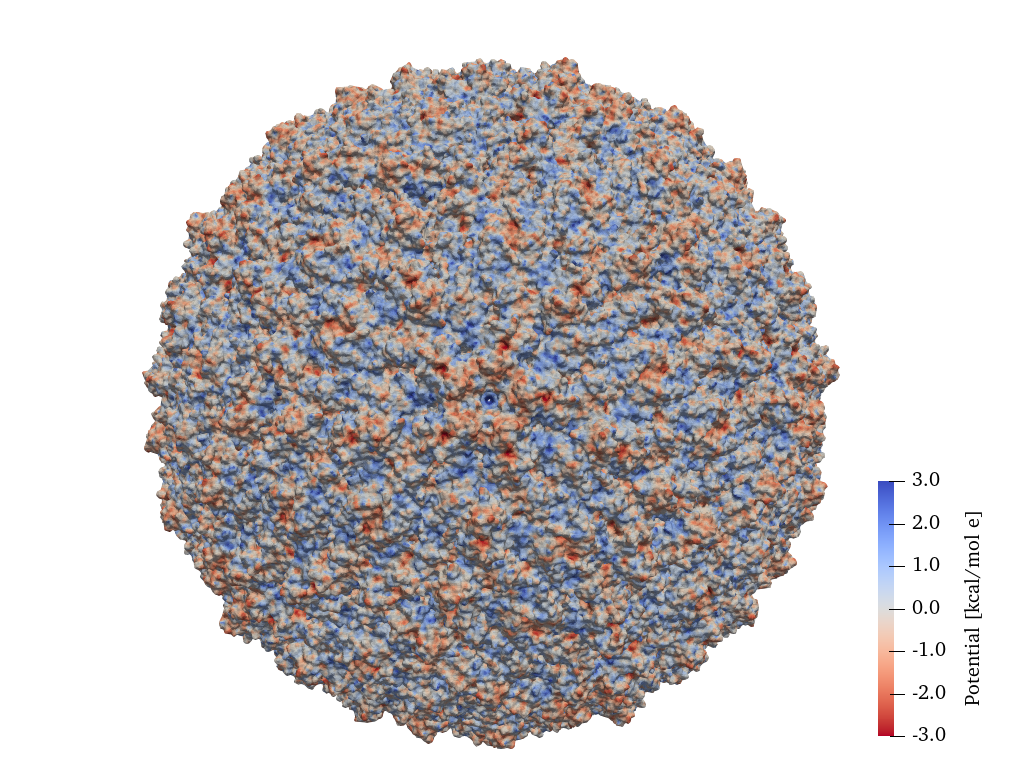
\includegraphics[width=\linewidth]{6CO8_potential.png} 
    \caption{Surface electrostatic potential of Zika virus. Visualization generated using ParaView.}
    \label{fig:6CO8_potential}
\end{figure*}

Table \ref{tab:6CO8_result} summarizes the results and performance.
Again, we confirmed that Juffer's formulation yields a well-conditioned system, which converged in 17 iterations and took less than 1.5 hours to solve.
By constrast, direct formulation took almost twice as long to converge.
As for assembly time, the gap between the two formulations becomes much bigger than all the previous cases.
As we explained before, it is because the sparse LU-decomposition in Juffer's formulation does not scale linearly with $N$, thus dominated the assembly time.

In this case, we also verified against \pygbe, a Python \bem library for biomolecular electrostatics.
Based on the solvation energy computed from \pygbe: $-117261.1$ [kcal/mol], the relative difference of our result is 0.6\% for direct formulation and 0.9\% for Juffer's formulation.
Figure \ref{fig:6CO8_potential} shows the calculated electrostatic potential.

\subsection{Reproducibility package}

Besides releasing our code with an open-source license, we spared no effort to maximize the reproducibility of this work via a ``repro-pack" in a version-control repository.
It contains all raw data from the experiments and post-processing scripts, which are sufficient to produce every result presented in this section.
The ``repro-pack" also provides driver and utility scripts should readers be interested in running these cases on their own hardware.
The meshes and pqr files are available on Zenodo...